\renewcommand{\tema}{Lección: Ondas y Óptica}

% ============================================================
%  SECCIÓN 1: CARACTERIZACIÓN DE ONDAS
% ============================================================

\section{Caracterización de Ondas}

\begin{seccion}
Una onda es una perturbación que se propaga en el espacio y transporta energía sin transportar materia. Cuando una piedra cae en un estanque, la superficie del agua sube y baja, pero el agua en sí no viaja hacia la orilla: lo que viaja es la perturbación. Este principio es fundamental para entender desde el sonido hasta la luz.
\end{seccion}

\subsection{Clasificación por la dirección de vibración}

\begin{seccion}
\begin{definicion}
\textbf{Onda transversal:} La perturbación oscila en dirección \textit{perpendicular} a la dirección de propagación.
\end{definicion}

\textbf{Ejemplos:} ondas en una cuerda tensa, ondas en la superficie del agua, luz y ondas electromagnéticas en general.

\vspace{0.3cm}

\begin{definicion}
\textbf{Onda longitudinal:} La perturbación oscila en dirección \textit{paralela} a la dirección de propagación. El medio se comprime y se rarifica alternativamente.
\end{definicion}

\textbf{Ejemplos:} el sonido en el aire, ondas sísmicas de tipo P, ondas en un resorte comprimido.
\end{seccion}


\begin{center}
    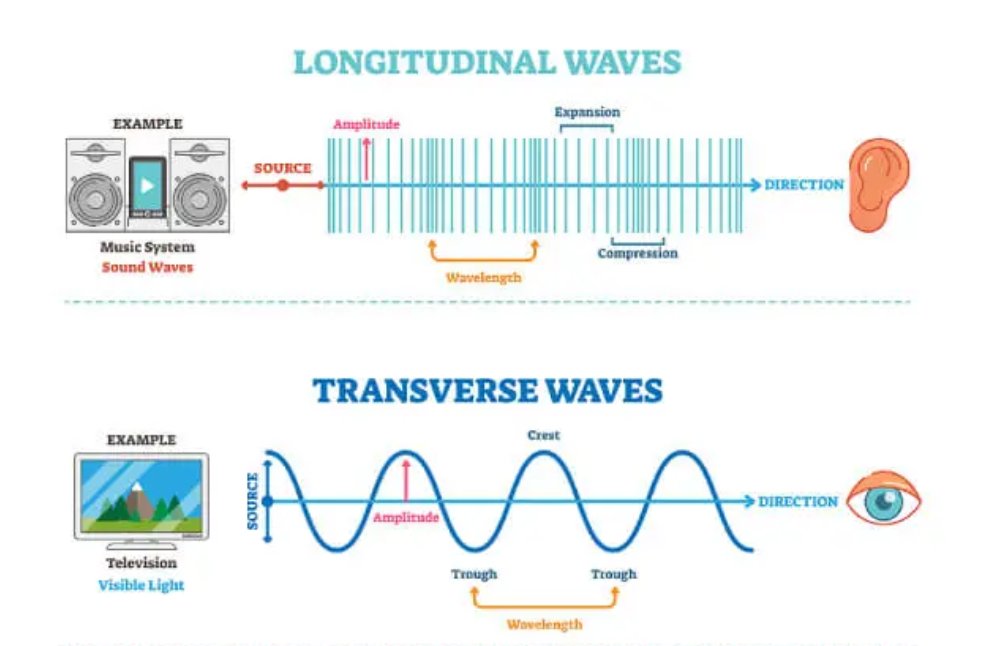
\includegraphics[width=0.7\textwidth]{CLASES/IMAGENES/longitudinales_transversales.png}
\end{center}
\newpage
\subsection{Parámetros que caracterizan una onda}

\begin{seccion}
Toda onda periódica queda completamente descrita por cinco parámetros. Conocer cualquier par de ellos permite deducir los demás a través de las relaciones que se presentan a continuación.

\begin{ecuacion}
\textbf{Frecuencia} ($f$): número de ciclos completos que ocurren por segundo.
$$f = \frac{\text{número de ciclos}}{\text{tiempo total}}$$
Unidad: hertz (Hz) $= \text{ciclos/s} = \text{s}^{-1}$
\end{ecuacion}

\begin{ecuacion}
\textbf{Periodo} ($T$): tiempo que tarda en completarse un ciclo. Es el recíproco de la frecuencia.
$$T = \frac{1}{f} \qquad \Longleftrightarrow \qquad f = \frac{1}{T}$$
Unidad: segundos (s)
\end{ecuacion}

\begin{ecuacion}
\textbf{Longitud de onda} ($\lambda$): distancia entre dos puntos consecutivos que están en la misma fase (por ejemplo, cresta con cresta, o valle con valle).

Unidad: metros (m)
\end{ecuacion}

\begin{ecuacion}
\textbf{Amplitud} ($A$): valor máximo del desplazamiento respecto a la posición de equilibrio. La amplitud determina la \textbf{intensidad} (energía) de la onda, no su velocidad ni su frecuencia.

Las unidades dependen de la naturaleza física de la onda: metros (m) para ondas mecánicas como el sonido o las ondas en una cuerda; volts por metro (V/m) para el campo eléctrico de una onda electromagnética; pascales (Pa) para la presión en una onda sonora.
\end{ecuacion}

\begin{ecuacion}
\textbf{Velocidad de propagación} ($v$): rapidez con que se desplaza la perturbación en el medio. Depende del medio, no de quien genera la onda.
$$v = \lambda \cdot f = \frac{\lambda}{T}$$
Unidad: metros por segundo (m/s)
\end{ecuacion}

\begin{nota}
\textbf{Nota:} Si la frecuencia aumenta y la velocidad se mantiene constante (mismo medio), la longitud de onda \textit{disminuye} en la misma proporción. Esta relación inversa entre $\lambda$ y $f$ es esencial para entender el espectro electromagnético.
\end{nota}
\end{seccion}

\subsubsection{Diagrama: Parámetros de una onda transversal}

\begin{center}
\begin{tikzpicture}[scale=1.1]

% Eje x
\draw[-{Stealth}, thick, color=azuloscuro] (-0.3,0) -- (9,0)
    node[right, font=\small] {distancia};
% Eje y
\draw[-{Stealth}, thick, color=azuloscuro] (0,-1.8) -- (0,2.3)
    node[above, font=\small] {desplazamiento};

% Onda
\draw[color=azulmedio, very thick, domain=0:8.5, samples=80]
    plot (\x, {1.4*sin(deg(3.14159*\x/2))});

% --- Amplitud ---
\draw[{Stealth}-{Stealth}, color=verdecorrecto, thick]
    (1.0, 0) -- (1.0, 1.4);
\node[right, font=\small, color=verdecorrecto] at (1.05, 0.7) {$A$};

% --- Longitud de onda (de cresta a cresta) ---
\draw[{Stealth}-{Stealth}, color=red!70!black, thick]
    (1.0, 1.7) -- (5.0, 1.7);
\node[above, font=\small, color=red!70!black] at (3.0, 1.7) {$\lambda$};
\draw[dashed, thin, color=red!70!black] (1.0,1.4) -- (1.0,1.7);
\draw[dashed, thin, color=red!70!black] (5.0,1.4) -- (5.0,1.7);

% --- Etiquetas cresta / valle ---
\node[above, font=\footnotesize, color=azulmedio] at (0.5, 1.4) {cresta};
\node[below, font=\footnotesize, color=azulmedio] at (3.0,-1.4) {valle};

% Línea de equilibrio
\draw[dashed, thin, color=gray] (-0.2,0) -- (8.8,0);
\node[left, font=\footnotesize, color=gray] at (-0.4,0) {equilibrio};

\end{tikzpicture}
\end{center}

\subsection{Ejercicios resueltos: parámetros de una onda}

\begin{seccion}

\textbf{Ejercicio 1.} Una onda tiene una frecuencia de 70 Hz y una longitud de onda de 3 m. ¿Cuál es su velocidad de propagación?

\begin{ecuacion}
\textbf{Datos:} $f = 70$ Hz, $\lambda = 3$ m \quad \textbf{Fórmula:} $v = \lambda \cdot f$

\textbf{Sustitución:}
$$v = 3 \text{ m} \times 70 \text{ Hz} = 210 \text{ m/s}$$
\end{ecuacion}

\vspace{0.4cm}

\textbf{Ejercicio 2.} Una persona parada en la orilla de un muelle observa que la cresta de una ola pasa cada 2 s. Si la distancia entre crestas es de 5.2 m, ¿cuál es la velocidad de las ondas superficiales?

\begin{ecuacion}
\textbf{Datos:} $T = 2$ s $\Rightarrow f = \dfrac{1}{T} = 0.5$ Hz, $\lambda = 5.2$ m

$$v = \lambda \cdot f = 5.2 \text{ m} \times 0.5 \text{ Hz} = 2.6 \text{ m/s}$$
\end{ecuacion}

\vspace{0.4cm}

\textbf{Ejercicio 3.} Una onda se propaga con velocidad $v$, frecuencia $f$ y longitud de onda $\lambda$. Si la frecuencia aumenta al doble y la velocidad permanece constante, ¿cuál es la nueva longitud de onda?

\begin{ecuacion}
De $v = \lambda \cdot f$ se desprende $\lambda = \dfrac{v}{f}$. Si la frecuencia se duplica ($f' = 2f$) con $v$ constante:
$$\lambda' = \frac{v}{2f} = \frac{\lambda}{2}$$
La longitud de onda se reduce a la mitad.
\end{ecuacion}

\begin{nota}
\textbf{Nota:} En los ejercicios anteriores, los datos están diseñados para producir resultados enteros o decimales simples. En el examen de admisión siempre será así: si el cálculo te da un número complicado, revisa si confundiste $f$ con $T$, o si olvidaste convertir unidades.
\end{nota}

\end{seccion}

% ============================================================
%  SECCIÓN 2: CAMBIOS EN LA TRAYECTORIA DE LAS ONDAS
% ============================================================

\begin{seccion}
Cuando una onda encuentra un obstáculo, una frontera entre medios o una apertura, su comportamiento cambia. Estos fenómenos no son exclusivos de un tipo de onda: ocurren con el sonido, con el agua y con la luz. Entenderlos en el contexto general de las ondas facilita mucho la comprensión de la óptica.
\end{seccion}

\subsection{Reflexión}

\begin{seccion}
\begin{definicion}
\textbf{Reflexión:} Una onda incide sobre una superficie y \textit{rebota} de regreso al mismo medio del que venía. La dirección del rebote sigue la \textbf{ley de reflexión}: el ángulo de incidencia es igual al ángulo de reflexión, ambos medidos respecto a la normal a la superficie.
\end{definicion}

$$\theta_i = \theta_r$$

\textbf{Ejemplos cotidianos:}
\begin{itemize}
    \item El eco es la reflexión del sonido en una pared o un acantilado.
    \item La imagen en un espejo es la reflexión de la luz en una superficie lisa.
    \item El radar aprovecha la reflexión de ondas de radio en los aviones.
\end{itemize}
\end{seccion}

\subsubsection{Diagrama: Reflexión de una onda}

\begin{center}
\begin{tikzpicture}[scale=1.1]

% Superficie reflectante
\draw[very thick, color=azuloscuro] (-3,0) -- (3,0);
% Rayado inferior (medio 2)
\foreach \x in {-2.8,-2.2,...,2.8} {
    \draw[thin, color=gray!50] (\x, 0) -- (\x-0.4, -0.4);
}

% Normal
\draw[dashed, color=gray, thick] (0,-1.2) -- (0,2.0);
\node[right, font=\footnotesize, color=gray] at (0.05,1.7) {normal};

% Rayo incidente
\draw[-{Stealth}, very thick, color=azulmedio]
    (-2.2, 1.8) -- (0,0);
\node[left, font=\small, color=azulmedio] at (-1.7,1.3) {rayo incidente};

% Rayo reflejado
\draw[-{Stealth}, very thick, color=verdecorrecto]
    (0,0) -- (2.2, 1.8);
\node[right, font=\small, color=verdecorrecto] at (1.7,1.3) {rayo reflejado};

% Ángulo incidente
\draw[color=azulmedio, thin] (0,0.7) arc (90:141:0.7);
\node[font=\footnotesize, color=azulmedio] at (-0.5,0.85) {$\theta_i$};

% Ángulo reflejado
\draw[color=verdecorrecto, thin] (0,0.7) arc (90:39:0.7);
\node[font=\footnotesize, color=verdecorrecto] at (0.5,0.85) {$\theta_r$};

\end{tikzpicture}
\end{center}

\subsection{Refracción}

\begin{seccion}
\begin{definicion}
\textbf{Refracción:} Una onda pasa de un medio a otro con diferente velocidad de propagación y, al hacerlo, \textit{cambia de dirección}. El cambio de dirección ocurre porque un lado del frente de onda viaja más rápido que el otro al cruzar la frontera.
\end{definicion}


\textbf{Ejemplo clásico:} La cuchara que parece ``rota'' dentro de un vaso de agua. La luz que viene de la cuchara cambia de velocidad al pasar del agua al aire, lo cual la desvía y produce la ilusión visual.
\end{seccion}

\subsubsection{Diagrama: Refracción de una onda}

\begin{center}
\begin{tikzpicture}[scale=1.15]

% ---- Medio superior (más rápido, v1) ----
\fill[azulmedio!8] (-3.5, 0) rectangle (3.5, 3.0);
\node[font=\small, color=azuloscuro] at (-2.8, 0.6) {Medio 1};
\node[font=\footnotesize, color=azuloscuro] at (-2.1, 0.2) {(velocidad $v_1$, mayor)};

% ---- Medio inferior (más lento, v2) ----
\fill[azulmedio!22] (-3.5, -2.8) rectangle (3.5, 0);
\node[font=\small, color=azuloscuro] at (-2.8, -0.3) {Medio 2};
\node[font=\footnotesize, color=azuloscuro] at (-2.1, -0.7) {(velocidad $v_2$, menor)};

% ---- Superficie de separación ----
\draw[very thick, color=azuloscuro] (-3.5, 0) -- (3.5, 0);
% Rayado de separación
\foreach \x in {-3.3,-2.9,...,3.3} {
    \draw[gray!40, thin] (\x, 0) -- (\x+0.3, -0.3);
}

% ---- Normal ----
\draw[dashed, gray, thick] (0, -2.6) -- (0, 2.8);
\node[right, font=\footnotesize, color=gray] at (0.05, 2.5) {normal};

% ---- Rayo incidente ----
\draw[-{Stealth}, very thick, color=azulmedio]
    (-2.4, 2.6) -- (0, 0);
\node[left, font=\small, color=azulmedio] at (-1.7, 1.8) {rayo incidente};

% ---- Rayo reflejado (tenue) ----
\draw[-{Stealth}, thick, color=azulmedio!50, dashed]
    (0, 0) -- (2.4, 2.6);
\node[right, font=\footnotesize, color=azulmedio!70] at (1.8, 1.8) {reflejado};

% ---- Rayo refractado (más cerca de la normal) ----
\draw[-{Stealth}, very thick, color=verdecorrecto]
    (0, 0) -- (1.4, -2.6);
\node[right, font=\small, color=verdecorrecto] at (1.0, -1.6) {rayo refractado};

% ---- Ángulo de incidencia ----
\draw[color=azulmedio, thin] (0, 0.8) arc (90:132:0.8);
\node[font=\footnotesize, color=azulmedio] at (-0.55, 1.0) {$\theta_1$};

% ---- Ángulo de refracción ----
\draw[color=verdecorrecto, thin] (0,-0.8) arc (270:297:0.8);
\node[font=\footnotesize, color=verdecorrecto] at (0.3, -1.05) {$\theta_2$};

% ---- Nota: ángulo se acerca a la normal ----
\node[font=\footnotesize, color=gray!80] at (2.5, -0.5)
    {$\theta_2 < \theta_1$};
\node[font=\footnotesize, color=gray!80] at (2.5, -0.9)
    {(medio más lento)};

\end{tikzpicture}
\end{center}

\subsection{Interferencia}

\begin{seccion}
\begin{definicion}
\textbf{Interferencia:} Cuando dos o más ondas se superponen en el mismo punto del medio, sus desplazamientos se \textit{suman algebraicamente}. El resultado puede ser una onda más intensa, menos intensa, o incluso nula.
\end{definicion}

\begin{ecuacion}
\textbf{Interferencia constructiva:} Las ondas llegan en fase (cresta con cresta, valle con valle). La amplitud resultante es la \textit{suma} de las amplitudes individuales.
$$A_{\text{total}} = A_1 + A_2$$
\textbf{Efecto:} la onda se amplifica.
\end{ecuacion}

\begin{ecuacion}
\textbf{Interferencia destructiva:} Las ondas llegan en contrafase (cresta con valle). La amplitud resultante es la \textit{diferencia} de las amplitudes.
$$A_{\text{total}} = A_1 - A_2$$
\textbf{Efecto:} la onda se reduce o se cancela completamente (si $A_1 = A_2$).
\end{ecuacion}

\textbf{Ejemplos:}
\begin{itemize}
    \item Los audífonos con cancelación activa de ruido usan interferencia destructiva para eliminar ruido externo.
    \item Los colores iridiscentes en burbujas de jabón y en alas de mariposa se deben a interferencia constructiva y destructiva de la luz reflejada en capas delgadas.
\end{itemize}
\end{seccion}

\subsubsection{Diagrama: Interferencia constructiva y destructiva}

\begin{center}
\begin{tikzpicture}[scale=0.95]

% ================================================================
% TÍTULO CONSTRUCTIVA
% ================================================================
\node[font=\bfseries\normalsize, color=azulmedio] at (4.5, 6.8) {Interferencia constructiva};

% --- Onda 1 (azul) ---
\draw[azulmedio, thick, domain=0:9, samples=80]
    plot (\x, {0.8*sin(deg(2*3.14159*\x/3.0)) + 5.5});
\draw[dashed, gray!60, thin] (0, 5.5) -- (9, 5.5);
\node[left, font=\small, color=azulmedio] at (0, 5.5) {$A_1$};

% --- Onda 2 (verde, misma fase) ---
\draw[verdecorrecto, thick, domain=0:9, samples=80]
    plot (\x, {0.6*sin(deg(2*3.14159*\x/3.0)) + 4.0});
\draw[dashed, gray!60, thin] (0, 4.0) -- (9, 4.0);
\node[left, font=\small, color=verdecorrecto] at (0, 4.0) {$A_2$};

% --- Resultante (rojo, amplitud = A1+A2) ---
\draw[red!70!black, very thick, domain=0:9, samples=80]
    plot (\x, {1.4*sin(deg(2*3.14159*\x/3.0)) + 2.2});
\draw[dashed, gray!60, thin] (0, 2.2) -- (9, 2.2);
\node[left, font=\small, color=red!70!black] at (0, 2.2) {$A_1{+}A_2$};


% ================================================================
% TÍTULO DESTRUCTIVA
% ================================================================
\node[font=\bfseries\normalsize, color=azulmedio] at (4.5, 0.4) {Interferencia destructiva};

% --- Onda 1 (azul) ---
\draw[azulmedio, thick, domain=0:9, samples=80]
    plot (\x, {0.8*sin(deg(2*3.14159*\x/3.0)) - 0.8});
\draw[dashed, gray!60, thin] (0, -0.8) -- (9, -0.8);
\node[left, font=\small, color=azulmedio] at (0, -0.8) {$A_1$};

% --- Onda 2 (verde, desfase 180$^\circ$) ---
\draw[verdecorrecto, thick, domain=0:9, samples=80]
    plot (\x, {0.8*sin(deg(2*3.14159*\x/3.0 + 180/(2*pi))) - 2.5});
\draw[dashed, gray!60, thin] (0, -2.5) -- (9, -2.5);
\node[left, font=\small, color=verdecorrecto] at (0, -2.5) {$A_2$};

% --- Resultante (línea plana en 0) ---
\draw[red!70!black, very thick] (0, -3.7) -- (9, -3.7);
\draw[dashed, gray!60, thin] (0, -3.7) -- (9, -3.7);
\node[left, font=\small, color=red!70!black] at (0, -3.7) {$0$};

\end{tikzpicture}
\end{center}

\subsection{Difracción}

\begin{seccion}
\begin{definicion}
\textbf{Difracción:} Una onda se \textit{dobla} alrededor de los bordes de un obstáculo o al pasar por una apertura estrecha, propagándose hacia regiones que geométricamente estarían en la ``sombra'' del obstáculo.
\end{definicion}

Es importante recordar que la difracción es significativa cuando el tamaño del obstáculo o la apertura es comparable a la longitud de onda. Si el obstáculo es mucho más grande que $\lambda$, la onda prácticamente no se dobla (se comporta como un rayo rectilíneo).

\textbf{Ejemplos:}
\begin{itemize}
    \item El sonido se difracta fácilmente alrededor de las esquinas de los edificios (longitudes de onda de centímetros a metros), por eso escuchas música aunque no estés en línea directa con la bocina.
    \item La luz tiene longitudes de onda muy pequeñas ($\sim$500 nm), por lo que apenas se difracta con objetos cotidianos y viaja en línea recta. Sin embargo, sí se difracta en rendijas muy finas (experimento de Young).
    \item Las señales de radio AM (longitudes de onda de cientos de metros) se difractan alrededor de montañas enteras.
\end{itemize}
\end{seccion}

\subsubsection{Diagrama: Difracción por un obstáculo y por un orificio}


\begin{center}
    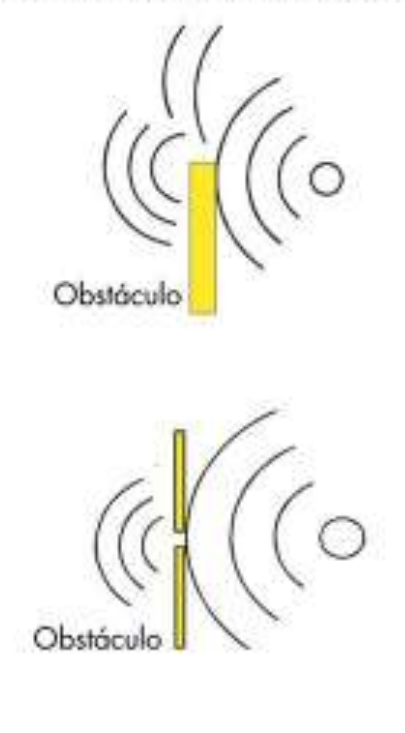
\includegraphics[width=0.20\textwidth]{CLASES/IMAGENES/difraccion.png}
\end{center}

\subsection{Amortiguación y transmisión de energía}

\begin{seccion}
\begin{definicion}
\textbf{Amortiguación:} A medida que una onda se propaga, parte de su energía se transfiere al medio o se disipa, lo que reduce progresivamente su amplitud. La onda no desaparece abruptamente: se debilita de forma gradual.
\end{definicion}

La energía de una onda es proporcional al cuadrado de su amplitud. Cuando la amplitud se reduce a la mitad, la energía transportada se reduce a una cuarta parte.

\textbf{Ejemplos prácticos:}
\begin{itemize}
    \item \textbf{Sonido en el aire:} La voz humana se percibe a pocos metros. Un sistema de megafonía compensa la amortiguación amplificando la señal en varios puntos del recorrido.
    \item \textbf{Ondas sísmicas:} Un terremoto genera ondas que viajan miles de kilómetros, pero su intensidad disminuye con la distancia. Por eso las ciudades alejadas del epicentro sienten el temblor con menor intensidad.
    \item \textbf{Señal de Wi-Fi:} Las paredes absorben parte de la energía de las microondas. A mayor número de paredes entre el router y el dispositivo, menor intensidad de señal.
    \item \textbf{Luz en el agua:} La luz solar penetra los primeros metros del océano con fuerza, pero a 200 metros de profundidad la oscuridad es casi total porque el agua absorbió prácticamente toda la energía.
    \item \textbf{Cuerdas de guitarra:} Después de puntear una cuerda, la vibración (y el sonido) se amortigua gradualmente hasta el silencio porque la energía se disipa como calor en la cuerda y en el aire circundante.
\end{itemize}
\end{seccion}

\subsubsection{Diagrama: Amortiguación de una onda}

\begin{center}
\begin{tikzpicture}[scale=1.0]

% Eje x
\draw[-{Stealth}, thick, color=azuloscuro] (-0.3, 0) -- (10.5, 0)
    node[right, font=\small] {distancia de propagación};
% Eje y
\draw[-{Stealth}, thick, color=azuloscuro] (0, -2.5) -- (0, 2.8)
    node[above, font=\small] {amplitud};

% Onda amortiguada: A(x)*sin(kx), con A(x) = 2.2*exp(-0.22*x)
\draw[azulmedio, very thick, domain=0:10, samples=80]
    plot (\x, {2.2*exp(-0.22*\x)*sin(deg(2.8*\x))});

% Envolvente superior
\draw[red!60!black, dashed, thick, domain=0:10, samples=60]
    plot (\x, { 2.2*exp(-0.22*\x)});
% Envolvente inferior
\draw[red!60!black, dashed, thick, domain=0:10, samples=60]
    plot (\x, {-2.2*exp(-0.22*\x)});

% Etiqueta envolvente
\node[right, font=\footnotesize, color=red!60!black] at (0.1, 2.3)
    {envolvente};

% Flechas de amplitud en distintas posiciones
\draw[{Stealth}-{Stealth}, verdecorrecto, thick]
    (0.55, 0) -- (0.55, {2.2*exp(-0.22*0.55)});
\node[right, font=\footnotesize, color=verdecorrecto] at (0.4, 1.0) {$A_0$};

\draw[{Stealth}-{Stealth}, verdecorrecto, thick]
    (3.7, 0) -- (3.7, {2.2*exp(-0.22*3.7)});
\node[right, font=\footnotesize, color=verdecorrecto] at (3.75, 0.55) {$A_1$};

\draw[{Stealth}-{Stealth}, verdecorrecto, thick]
    (7.0, 0) -- (7.0, {2.2*exp(-0.22*7.0)});
\node[right, font=\footnotesize, color=verdecorrecto] at (7.05, 0.3) {$A_2$};

% Relación de energía
\node[font=\footnotesize, color=gray] at (7.5, -2.2)
    {$A_0 > A_1 > A_2 \;\Rightarrow\; E_0 > E_1 > E_2$};

% Línea de equilibrio
\draw[dashed, gray!50, thin] (-0.2, 0) -- (10.3, 0);

\end{tikzpicture}
\end{center}

% ============================================================
%  FORMULARIO FINAL
% ============================================================

\section*{Formulario}

\begin{nota}

\textbf{Relación frecuencia-periodo:}
$$T = \frac{1}{f} \qquad \Longleftrightarrow \qquad f = \frac{1}{T}$$

\vspace{0.3cm}

\textbf{Velocidad de propagación:}
$$v = \lambda \cdot f = \frac{\lambda}{T}$$

\vspace{0.3cm}

\textbf{Longitud de onda (despejada):}
$$\lambda = \frac{v}{f} = v \cdot T$$

\vspace{0.3cm}

\textbf{Ley de reflexión:}
$$\theta_i = \theta_r$$

\vspace{0.3cm}

\textbf{Interferencia constructiva} (ondas en fase):
$$A_{\text{total}} = A_1 + A_2$$

\vspace{0.3cm}

\textbf{Interferencia destructiva} (ondas en contrafase):
$$A_{\text{total}} = |A_1 - A_2|$$

\vspace{0.3cm}

\textbf{Condición de difracción significativa:}
$$d \approx \lambda$$
donde $d$ es el tamaño del obstáculo o la apertura y $\lambda$ es la longitud de onda.

\vspace{0.3cm}

\textbf{Relación energía-amplitud:}
$$E \propto A^2$$
Si la amplitud se reduce a la mitad, la energía se reduce a una cuarta parte.

\end{nota}